%!TEX root = /Users/louis/Documents/PhD/Deliverables/Thesis/thesis.tex

\chapter{Evaluation}
\label{Evaluation}

%The evaluation chapter will outline our evaluation method and results, including the impact and limitations of our research; and discuss the extent to which the requirements identified in the analysis chapter have been fulfilled. Evaluation will be conducted in three ways: application of our structures and processes in a case study; publication of our research in academic journals, international conferences and workshops; and assessing the contribution made when delivering our work through an Eclipse research incubation project.

\section{Evaluation Measures}

%!TEX root = /Users/louis/Documents/PhD/Deliverables/Thesis/thesis.tex

\subsection{Case Study}
% We will apply our structures and processes to the Eclipse Generative Modelling Framework (GMF) project \cite{gronback06gmf}. GMF allows the definition of graphical concrete syntax for metamodels. GMF prescribes a model-driven approach: Users of GMF define concrete syntax as a model, which is used to generate a graphical editor. In fact, five models are used together to define a single editor using GMF.

% GMF defines the metamodels for graphical, tooling and mapping definition models; and for generator models. The metamodels have changed considerably during the development of GMF. Some changes have caused inconsistency with GMF models. Presently, migration is encoded in Java. Gronback has stated\footnote{Private communication, 2008.} that the migration code is being ported to QVT (a model-to-model transformation language) as the Java code is difficult to maintain.

% We identified GMF as the most appropriate candidate for the analysis phase of our research. Consequently, we decided to reserve GMF for the evaluation of our work.


%!TEX root = /Users/louis/Documents/PhD/Deliverables/Thesis/thesis.tex

\subsection{Collaborative Case Study}
%!TEX root = /Users/louis/Documents/PhD/Deliverables/Thesis/thesis.tex
\section[Evaluating Co-Evolution Tools with an Example from UML][Evaluating Co-Evolution Tools (UML)]{Evaluating Co-Evolution Tools with an Example from UML}
\label{sec:ttc}
In contrast to the previous section, which compared Flock to three co-evolution tools, the evaluation performed in this section compares Flock with model-to-model transformation tools. As discussed in Chapter~\ref{Analysis}, model migration can be regarded as a specialisation of model-to-model transformation. Chapter~\ref{Implementation} introduces Flock, a language tailored for model migration. This section compares Flock with other model-to-model transformation languages, and explores the benefits and drawbacks of treating model migration and model-to-model transformation as separate model management operations, as proposed in this thesis and by \cite{sprinkle03thesis}.

The author participated in the 2010 edition of the Transformation Tools Contest (TTC), a workshop series that seeks to compare and contrast tools for performing model and graph transformation. At TTC 2010\footnote{\url{http://www.planet-research20.org/ttc2010/index.php?Itemid=132}}, two rounds of submissions were invited: cases (transformation problems, three of which are selected by the workshop organisers) and solutions to the selected cases. The author submitted a case based on a model migration problem from a real-world example of metamodel evolution. Nine solutions were submitted for the case, including one by the author, which used Flock.

Compared to the evaluation described in Section~\ref{sec:collaborative_comparison}, the evaluation in this section compares Flock to a wider range of tools (model and graph transformation tools, and not just model migration tools). The remainder of this section describes the model migration case (Section~\ref{subsec:ttc_case}), the Flock solution (Section~\ref{subsec:ttc_solution}), and reports the results of the workshop in which the solutions were compared and scored by the organisers and participants.


\subsection{Model Migration Case}
\label{subsec:ttc_case}
To compare Flock with other transformation tools for specifying model migration, the author submitted a case to TTC based on the evolution of the UML. The way in which activity diagrams are modelled in the UML changed significantly between versions 1.4 and 2.1 of the specification. In the former, activities were defined as a special case of state machines, while in the latter they are defined with a more general semantic base\footnote{A variant of generalised coloured Petri nets.} \cite{selic05uml2}.

The remainder of this section briefly introduces UML activity diagrams, describes their evolution, and discusses the way in which solutions were assessed. Section~\ref{subsec:uml_activity_diagrams} describes the metamodel evolution in more detail. The work presented in this section is based on the case submitted to TTC 2010 \cite{rose10ttc_case}. 

\subsubsection{Activity Diagrams in UML}
Activity diagrams are used for modelling lower-level behaviours, emphasising sequencing and co-ordination conditions. They are used to model business processes and logic \cite{uml22}. Figure~\ref{fig:activity} shows an activity diagram for filling orders. The diagram is partitioned into three \emph{swimlanes}, representing different organisational units. \emph{Activities} are represented with rounded rectangles and \emph{transitions} with directed arrows. \emph{Fork} and \emph{join} nodes are specified using a solid black rectangle. \emph{Decision} nodes are represented with a diamond. Guards on transitions are specified using square brackets. For example, in Figure~\ref{fig:activity} the transition to the restock activity is guarded by the condition \texttt{[not in stock]}. Text on transitions that is not enclosed in square brackets represents a trigger event. In Figure~\ref{fig:activity}, the transition from the restock activity occurs on receipt of the asynchronous signal called \texttt{receive stock}. Finally, the transitions between activities might involve interaction with objects. In Figure~\ref{fig:activity}, the Fill Order activity leads to an interaction with an object called \texttt{Filled Object}. 

\begin{figure}[htbp]
  \centering
  \includegraphics*[viewport=75 230 585 800,width=13cm]{6.Evaluation/images/activity.pdf}
  \caption[Activity model in UML 1.4.]{Activity model in UML 1.4, taken from \cite{rose10ttc_case} and based on \cite[pg3-165]{uml14}.}
  \label{fig:activity}
\end{figure}

Between versions 1.4 and 2.2 of the UML specification, the metamodel for activity diagrams has changed significantly. The \cc sequel summarises most of the changes, and further details can be found in the UML 1.4 \cite{uml14} and UML 2.2 \cite{uml22} specifications.

\subsubsection{Evolution of Activity Diagrams}
Figures~\ref{fig:uml14} and \ref{fig:uml22} are simplifications of the activity diagram metamodels from versions 1.4 and 2.2 of the UML specification, respectively. In the interest of clarity, some features and abstract classes have been removed from Figures~\ref{fig:uml14} and \ref{fig:uml22}.

Some differences between Figures~\ref{fig:uml14} and \ref{fig:uml22} are: activities have been changed such that they comprise nodes and edges, actions replace states in UML 2.2, and the subtypes of control node replace pseudostates.

\begin{figure}[htbp]
  \centering
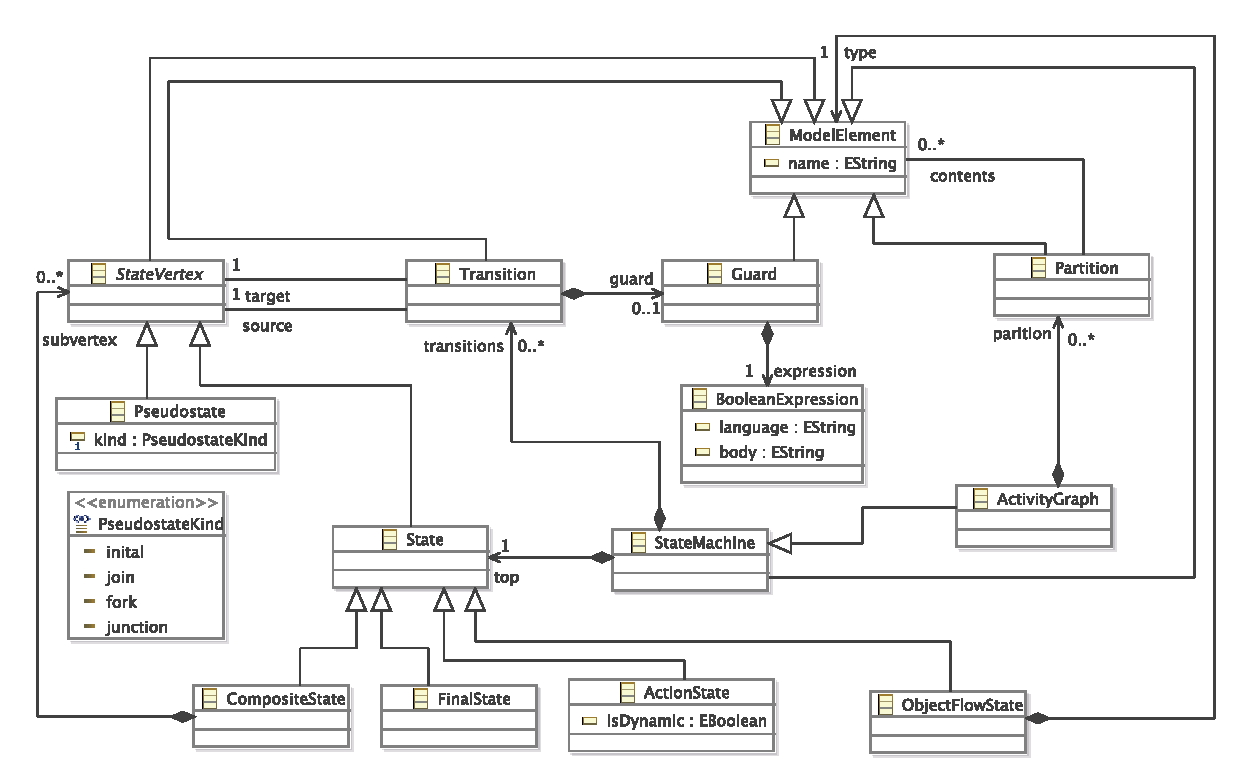
\includegraphics[width=12cm]{A.3.MigrationStrategies/images/uml/activity_diagrams_before.pdf}
  \caption[UML 1.4 Activity Graphs]{UML 1.4 Activity Graphs (based on \cite{uml14}).}
  \label{fig:uml14}
\end{figure} 

\begin{figure}[htbp]
  \centering
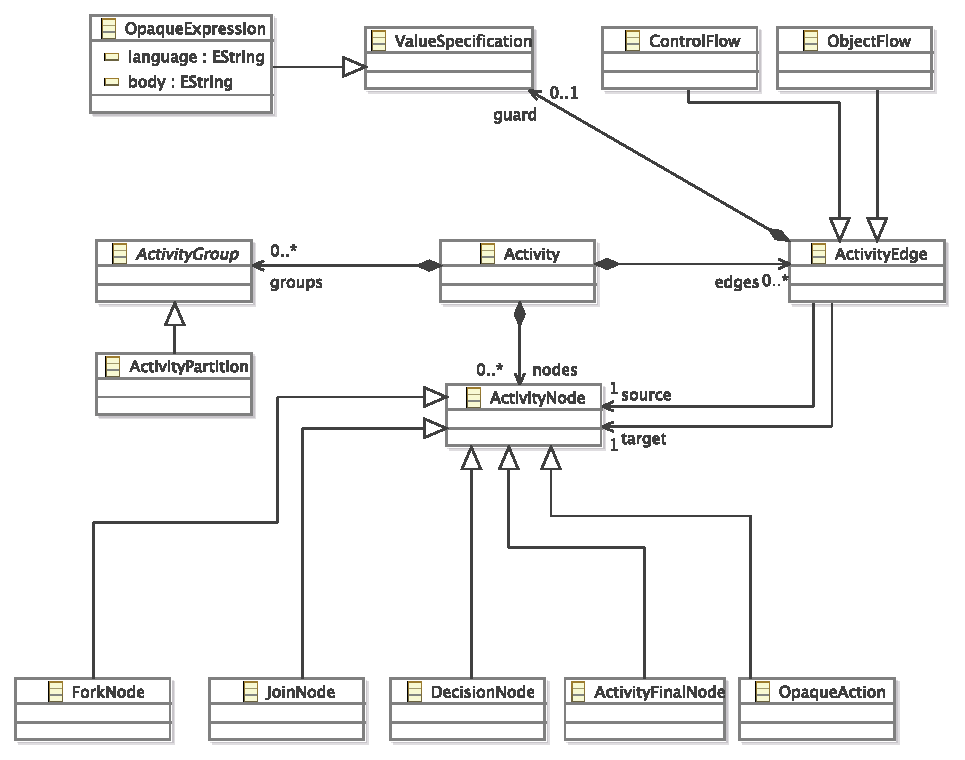
\includegraphics[width=12cm]{A.3.MigrationStrategies/images/uml/activity_diagrams_after.pdf}
  \caption[UML 2.2 Activity Diagrams]{UML 2.2 Activity Diagrams (based on \cite{uml22}).}
  \label{fig:uml22}
\end{figure}

To facilitate the comparison of solutions, the model shown in Figure~\ref{fig:activity} was used. Solutions migrated the activity diagram shown in Figure~\ref{fig:activity} -- which conforms to UML 1.4 -- to conform to UML 2.2. The UML 1.4 model, the migrated UML 2.2 model, and the UML 1.4 and 2.2 metamodels are available from\footnote{\url{http://www.cs.york.ac.uk/~louis/ttc/}}.

Submissions were evaluated using the following criteria, which were decided in advance by the author and the workshop organisers:

\begin{itemize}
	\item \textbf{Correctness}: Does the transformation produce a model equivalent to the migrated UML 2.2. model included in the case resources?
	\item \textbf{Conciseness}: How much code is required to specify the transformation? (Sprinkle \cc and Karsai propose that the amount of effort required to codify migration should be directly proportional to the number of changes between original and evolved metamodel \cite{sprinkle04domain}).
		\item \textbf{Clarity}: How easy is it to read and understand the used transformation? (For example, is a well-known or standardised language?)
		\item \textbf{Appropriateness}: How much effort is required to adapt the tool in providing a solution?
		\item \textbf{Tool maturity}: To what extent can the tool be used by people other than the developer? 
		\item \textbf{Reproducibility}: Can the solution be reproduced on another machine?\footnote{Participants were invited to install their tools and solutions on virtual machines, which would later be made accessible via the workshop proceedings.}
		\item \textbf{Extensions}: Which of the case extensions (described below) were implemented in the solution?
\end{itemize}

To further distinguish between solutions, three extensions to the core task were proposed. The first extension was added after the case was submitted, and was proposed by the workshop organisers and the solution authors. The second and third extension were included in the case by the author. 

\subsubsection{Extension 1: Alternative Object Flow State Migration Semantics}
\label{sub:object_flow_states}
Following the submission of the case to the competition, discussion on the TTC forums\footnote{\url{http://planet-research20.org/ttc2010/index.php?option=com_community&view=groups&task=viewgroup&groupid=4&Itemid=150} (registration required)} revealed an ambiguity in the UML 2.2 specification indicating that the migration semantics for the ObjectFlowState UML 1.4 concept are not clear from the UML 2.2 specification. The case was revised to incorporate both the original semantics (suggested by the author and described above) and an alternative semantics (suggested by a workshop participant via the TTC forums) for migrating \texttt{Ob\-je\-ctFl\-owSt\-a\-t\-es}. The alternative semantics are now described.

\textbf{In the core task} described above, instances of \texttt{Ob\-je\-ctFl\-owSt\-a\-te} were migrated to instances of \texttt{Ob\-je\-ctNo\-de}. Any instances of \texttt{Tr\-an\-si\-ti\-on} that had an \texttt{Ob\-je\-ctFl\-owSt\-a\-te} as their source or target were migrated to instances of \texttt{Ob\-je\-ctFl\-ow}. Figure~\ref{fig:ofs_to_node} shows an example application of this migration semantics. Structures such as the one shown in Figure~\ref{fig:ofs_to_node_before} are migrated to an equivalent structure shown in Figure~\ref{fig:ofs_to_node_after}. The \texttt{Tr\-an\-si\-ti\-on}s, \texttt{t1} and \texttt{t2}, are migrated to instances of \texttt{Ob\-je\-ctFl\-ow}. Likewise, the instance of \texttt{Ob\-je\-ctFl\-owSt\-a\-te}, \texttt{s2}, is migrated to an instance of \texttt{Ob\-je\-ctNo\-de}.

\begin{figure}[htbp]
	\centering
	\subfigure[ObjectFlowState structure in UML 1.4]
	{
	    \label{fig:ofs_to_node_before}
	    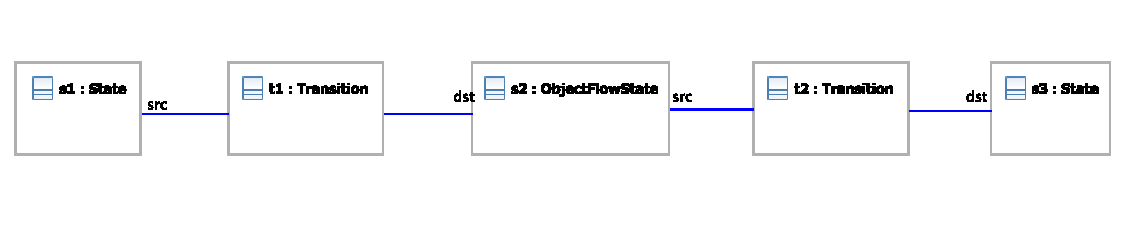
\includegraphics[height=2.5cm]{6.Evaluation/images/ttc/core_before.pdf}
	}
	\subfigure[Equivalent ObjectNode structure in UML 2.2]
	{
	    \label{fig:ofs_to_node_after}
	    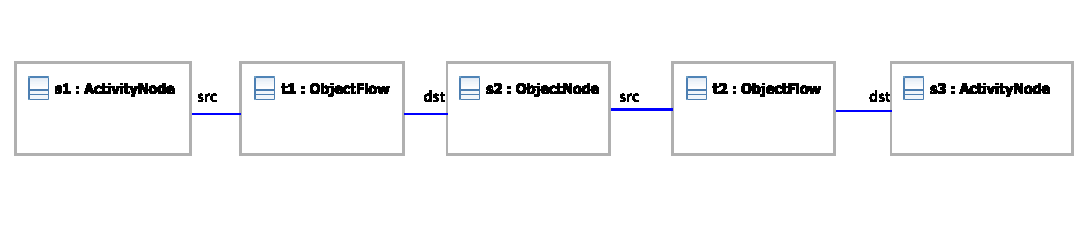
\includegraphics[height=2.5cm]{6.Evaluation/images/ttc/core_after.pdf}
	}
	\caption{Migrating Actions for the Core Task}
\label{fig:ofs_to_node}
\end{figure}


\textbf{This extension} considered an alternative migration semantics for ObjectFlowState. For this extension, instances of \texttt{Ob\-je\-ctFl\-owSt\-a\-te} (and any connected \texttt{Tr\-an\-si\-ti\-on}s) were migrated to instances of  \texttt{Ob\-je\-ctFl\-ow}, as shown in Figure~\ref{fig:ofs_to_flow} in which the UML 2.2 \texttt{Ob\-je\-ctFl\-ow}, \texttt{f1}, replaces \texttt{t1}, \texttt{t2} and \texttt{s2}.

\begin{figure}[htbp]
	\centering
	\subfigure[ObjectFlowState structure in UML 1.4]
	{
	    \label{fig:ofs_to_flow_before}
	    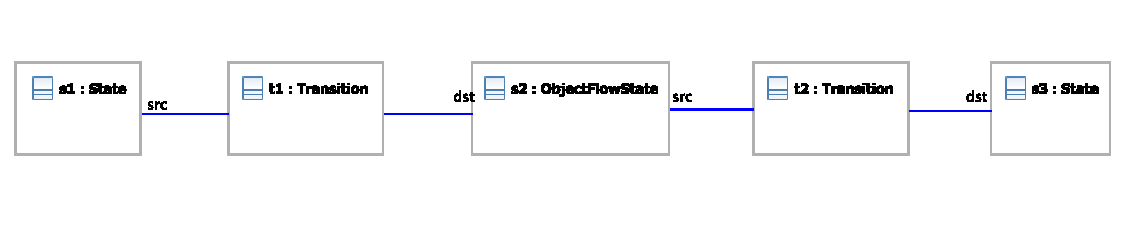
\includegraphics[height=2.5cm]{6.Evaluation/images/ttc/core_before.pdf}
	}
	\subfigure[Equivalent ObjectFlow structure in UML 2.2]
	{
	    \label{fig:ofs_to_flow_after}
	    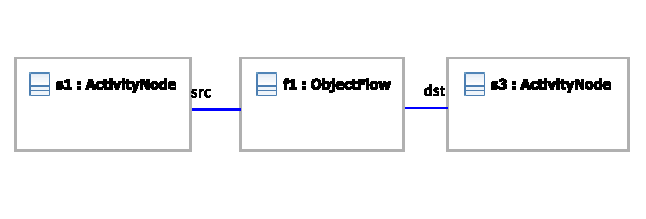
\includegraphics[height=2.5cm]{6.Evaluation/images/ttc/ext_after.pdf}
	}
	\caption{Migrating Actions for Extension 1}
\label{fig:ofs_to_flow}
\end{figure}

\subsubsection{Extension 2: Concrete Syntax}
\label{sub:concrete_syntax}
The second extension relates to the appearance of activity diagrams. The UML specifications provide no formally defined metamodel for the concrete syntax of UML diagrams. However, some UML tools store diagrammatic information in a structured manner using XML or a modelling tool. For example, the Eclipse UML 2 tools\footnote{\url{http://www.eclipse.org/modeling/mdt/?project=uml2tools}} store diagrams as GMF \cite{gronback09emp} diagram models.

Submissions were invited to explore the feasibility of migrating the concrete syntax of the activity diagram shown in Figure~\ref{fig:activity} to the concrete syntax in their chosen UML 2 tool. To facilitate this, the case resources included an ArgoUML project\footnote{\url{http://argouml.tigris.org/}} containing the activity diagram shown in Figure~\ref{fig:activity}.

\subsubsection{Extension 3: XMI}
\label{sub:xmi}
The UML specifications \cite{uml14,uml22} indicate that UML models should be stored using XMI. However, because XMI has evolved at the same time as UML, UML 1.4 tools most likely produce XMI of a different version to UML 2.2 tools. For instance, ArgoUML produces XMI 1.2 for UML 1.4 models, while the Eclipse UML2 tools produce XMI 2.1 for UML 2.2.

As an extension to the core task, submissions were invited to consider how to migrate a UML 1.4 model represented in XMI 1.x to a UML 2.1 model represented in XMI 2.x. To facilitate this, the UML 1.4 model shown in Figure~\ref{fig:activity} was made available in XMI 1.2 as part of the case resources.

Following the submission of the case, Tom Morris, the project leader for ArgoEclipse and a committer on ArgoUML, encouraged solutions to consider the extension described above. ArgoUML cannot, at present, migrate models from UML 1 to UML 2.  On the TTC forums, Morris stated that ``We have nothing available to fill this hole currently, so any contributions would be hugely valuable.  Not only would achieve academic fame and glory from the contest, but you'd get to see your code benefit users of one of the oldest (10+ yrs) open source UML modeling tools.'' \footnote{\url{http://www.planet-research20.org/ttc2010/index.php?option=com_community&view=groups&task=viewdiscussion&groupid=4&topicid=20&Itemid=150} (registration required)}

\subsection{Model Migration Solution in Epsilon Flock}
\label{subsec:ttc_solution}
This section describes a Flock solution for migrating UML activity diagrams in response to the evolution described above. The solution was developed by the author, and, at the workshop, compared with migration strategies written in other languages. The workshop participants and organisers rated each tool.

The Flock migration strategy was developed in an iterative and incremental manner, using the following process, starting with an empty migration strategy:

\begin{enumerate}
	\item Execute Flock on the original model, producing a migrated model.
	\item Compare the migrated model with the reference model provided in the case resources.
	\item Change the Flock migration strategy.
	\item Repeat until the migrated and reference models were the same.
\end{enumerate}

The remainder of this section presents the Flock solution in an incremental manner. The code listings in this section show only those rules relevant to the iteration being discussed.

\subsubsection{Actions, Transitions and Final States}
Development of the migration strategy began by executing an empty Flock migration strategy on the original model. Because Flock automatically copies model elements that have not been affected by evolution, the resulting model contained \texttt{Ps\-eu\-do\-st\-at\-e}s and \texttt{Tr\-an\-si\-ti\-on}s, but none of the \texttt{Ac\-ti\-onSt\-a\-te}s from the original model. In UML 2.2 activities, \texttt{Op\-aq\-ueAc\-ti\-on}s replace \texttt{Ac\-ti\-onSt\-a\-te}s. Listing~\ref{lst:actions} shows the Flock code for changing \texttt{Ac\-ti\-onSt\-a\-te}s to corresponding \texttt{Op\-aq\-ueAc\-ti\-on}s.

\begin{lstlisting}[caption=Migrating Actions, label=lst:actions, language=Flock]
migrate ActionState to OpaqueAction
\end{lstlisting}

Next, similar rules were added to migrate instances of \texttt{FinalState} to instances of \texttt{ActivityFinalNode} and to migrate instances of \texttt{Transition} to \texttt{ControlFlow}, as shown in Listing~\ref{lst:final_states}.

\begin{lstlisting}[caption=Migrating FinalStates and Transitions, label=lst:final_states, language=Flock]
migrate FinalState to ActivityFinalNode
migrate Transition to ControlFlow
\end{lstlisting}

\subsubsection{Pseudostates}
Development continued by selecting further types of state that were not present in the migrated model, such as \texttt{Ps\-eu\-do\-st\-at\-es}s, which are not used in UML 2.2 activities. Instead, UML 2.2 activities use specialised \texttt{No\-de}s, such as \texttt{In\-it\-ialNo\-de}. Listing~\ref{lst:pseudostates} shows the Flock code used to change \texttt{Ps\-eu\-do\-st\-a\-te}s to corresponding \texttt{No\-de}s.

\begin{lstlisting}[caption=Migrating Pseudostates, label=lst:pseudostates, language=Flock]
migrate Pseudostate to InitialNode  when: original.kind = Original!PseudostateKind#initial
migrate Pseudostate to DecisionNode when: original.kind = Original!PseudostateKind#junction
migrate Pseudostate to ForkNode     when: original.kind = Original!PseudostateKind#fork
migrate Pseudostate to JoinNode     when: original.kind = Original!PseudostateKind#join
\end{lstlisting}

\subsubsection{Activities}
In UML 2.2, \texttt{Ac\-ti\-vi\-ty}s no longer inherit from state machines. As such, some of the features defined by \texttt{Ac\-ti\-vi\-ty} have been renamed. Specifically, \texttt{tr\-an\-si\-ti\-o\-ns} has become \texttt{ed\-g\-es} and \texttt{par\-ti\-ti\-o\-ns} has become \texttt{gr\-o\-u\-ps}. Furthermore, the states (or nodes in UML 2.2 parlance) of an \texttt{Ac\-ti\-vi\-ty} are now contained in a feature called \texttt{nodes}, rather than in the \texttt{su\-bv\-er\-t\-ex} feature of a composite state accessed via the \texttt{top} feature of \texttt{Ac\-ti\-vi\-ty}. The Flock migration rule shown in Listing~\ref{lst:activities} captured these changes.

\begin{lstlisting}[caption=Migrating ActivityGraphs, label=lst:activities, language=Flock]
migrate ActivityGraph to Activity {
	migrated.edge  = original.transitions.equivalent();
	migrated.group = original.partition.equivalent();
	migrated.node  = original.top.subvertex.equivalent();
}
\end{lstlisting}

Note that the rule in Listing~\ref{lst:activities} used the built-in \texttt{eq\-ui\-va\-le\-nt} operation to find migrated model elements from original model elements. As discussed in Section~\ref{sec:flock}, the \texttt{equ\-iv\-al\-e\-nt} operation invokes other migration rules where necessary and caches results to improve performance.

Next, a similar rule for migrating \texttt{Gu\-ar\-d}s was added. In UML 1.4, the the \texttt{gu\-a\-rd} feature of \texttt{Tr\-an\-si\-ti\-on} references a \texttt{Gu\-a\-rd}, which in turn references an \texttt{Ex\-pr\-es\-si\-on} via its \texttt{ex\-pr\-es\-si\-on} feature. In UML 2.2, the \texttt{gu\-a\-rd} feature of \texttt{Tr\-an\-si\-ti\-on} references an \texttt{Op\-aq\-ueEx\-pr\-es\-si\-on} directly. Listing~\ref{lst:guards} captures this in Flock.

\begin{lstlisting}[caption=Migrating Guards, label=lst:guards, language=Flock]
migrate Guard to OpaqueExpression {
	migrated.body.add(original.expression.body);
}

\end{lstlisting}


\subsubsection{Partitions}
In UML 1.4 activity diagrams, \texttt{Pa\-rt\-it\-i\-on} specifies a single containment reference for its \texttt{co\-nt\-en\-ts}. In UML 2.2 activity diagrams, partitions have been renamed to \texttt{ActivityPartition}s and specify two containment features for their contents, \texttt{ed\-g\-es} and \texttt{no\-d\-es}. Listing~\ref{lst:partitions} shows the rule used to migrate \texttt{Pa\-rt\-it\-i\-on}s to \texttt{Ac\-ti\-vi\-tyPa\-rt\-it\-i\-on}s in Flock. The body of the rule shown in Listing~\ref{lst:partitions} uses the \emph{collect} operation to segregate the \texttt{co\-nt\-en\-ts} feature of the original model element into two parts.

\begin{lstlisting}[caption=Migrating Partitions, label=lst:partitions, language=Flock]
migrate Partition to ActivityPartition {
	migrated.edges = original.contents.collect(e:Transition | e.equivalent());
	migrated.nodes = original.contents.collect(n:StateVertex | n.equivalent());	
}
\end{lstlisting}


\subsubsection{ObjectFlows}
Finally, two rules were written for migrating model elements relating to object flows. In UML 1.4 activity diagrams, object flows are specified using \texttt{Ob\-je\-ctFl\-owSt\-a\-te}, a subtype of \texttt{St\-at\-eVe\-rt\-ex}. In UML 2.2 activity diagrams, object flows are modelled using a subtype of \texttt{ObjectNode}. In UML 2.2 flows that connect to and from \texttt{Ob\-je\-ctNo\-de}s must be represented with \texttt{Ob\-je\-ctFl\-ow}s rather than \texttt{Co\-nt\-rolFl\-ow}s.

Listing~\ref{lst:objectflows} shows the Flock rule used to migrate \texttt{Tr\-an\-si\-ti\-on}s to \texttt{Ob\-je\-ctFl\-ow}s. The rule applies for \texttt{Tr\-an\-si\-ti\-on}s whose source or target \texttt{St\-at\-eVe\-rt\-ex} is of type \texttt{Ob\-je\-ctFl\-owSt\-ate}.

\begin{lstlisting}[caption=Migrating ObjectFlows, label=lst:objectflows, language=Flock]
migrate ObjectFlowState to ActivityParameterNode

migrate Transition to ObjectFlow when: original.source.isTypeOf(ObjectFlowState) or original.target.isTypeOf(ObjectFlowState)
\end{lstlisting}

In addition to the core task, the Flock solution also approached two of the three extensions described in the case (Section~\ref{subsec:ttc_case}). The solutions to the extensions are now discussed.

\subsubsection{Alternative ObjectFlowState Migration Semantics}
The first extension required submissions to consider an alternative migration semantics for \texttt{Ob\-je\-ctFl\-owSt\-a\-te}, in which a single \texttt{Ob\-je\-ctFl\-ow} replaces each \texttt{Ob\-je\-ctFl\-owSt\-a\-te} and any connected \texttt{Tr\-an\-si\-ti\-on}s.

Listing~\ref{lst:objectflows2} shows the Flock source code used to migrate \texttt{Ob\-je\-ctFl\-owSt\-at\-es} (and connecting \texttt{Tr\-an\-si\-ti\-on}s) to a single \texttt{Ob\-je\-ctFl\-ow}. This rule was used instead of the two rules defined in Listing~\ref{lst:objectflows}. In the body of the rule shown in Listing~\ref{lst:objectflows2}, the \texttt{so\-ur\-ce} of the \texttt{Tr\-an\-si\-ti\-on} is copied directly to the \texttt{so\-u\-rce} of the \texttt{Ob\-je\-ctFl\-ow}. The \texttt{ta\-rg\-et} of the \texttt{Ob\-je\-ctFl\-ow} is set to the target of the first outgoing \texttt{Tr\-an\-si\-ti\-on} from the \texttt{Ob\-je\-ctFl\-owSt\-a\-te}. 

\begin{lstlisting}[caption=Migrating ObjectFlowStates to a single ObjectFlow, label=lst:objectflows2, language=Flock]
migrate Transition to ObjectFlow when: original.target.isTypeOf(ObjectFlowState) {
	migrated.source = original.source.equivalent();
	migrated.target = original.target.outgoing.first.target.equivalent();
}
\end{lstlisting}

Because, in this alternative semantics, \texttt{Ob\-je\-ctFl\-owSt\-a\-te}s are represented as edges rather than nodes, the partition migration rule was changed such that \texttt{Ob\-je\-ctFl\-owSt\-a\-te}s were not copied to the \texttt{no\-des} feature of \texttt{Pa\-rt\-it\-i\-on}s. To filter out the \texttt{Ob\-je\-ctFl\-owSt\-a\-te}s, line 3 of Listing~\ref{lst:partitions} was changed to include a reject statement, as shown on line 3 of Listing~\ref{lst:partitions2}.

\begin{lstlisting}[caption=Migrating Partitions without ObjectFlowStates, label=lst:partitions2, language=Flock]
migrate Partition to ActivityPartition {
	migrated.edges = original.contents.collect(e:Transition | e.equivalent());
	migrated.nodes = original.contents.reject(ofs:ObjectFlowState | true).collect(n:Original!StateVertex | n.equivalent());	
}
\end{lstlisting}

The complete source code listing for the Flock migration strategy is provided in Section~\ref{subsec:uml_activity_diagrams}.

\subsubsection{XMI}
\label{sec:xmi}
The second extension required submissions to migrate an activity graph conforming to UML 1.4 and encoded in XMI 1.2 to an equivalent activity graph conforming to UML 2.2 and encoded in XMI 2.1. The core task did not require submissions to consider changes to XMI (the model storage representation), but, in practice, this is a challenge to migration, as noted by Tom Morris on the TTC forums\footnote{\url{http://www.planet-research20.org/ttc2010/index.php?option=com_community&view=groups&task=viewdiscussion&groupid=4&topicid=20&Itemid=150} (registration required)}.

As discussed in Section~\ref{sec:flock}, Flock extends and reuses \changed{``is built atop'' changed to ``extends and reuses''} Epsilon, which includes a model connectivity layer (EMC). EMC provides a common interface for accessing and persisting models. Currently, EMC supports EMF (XMI 2.x), MDR (XMI 1.x), and plain XML models. To support migration between metamodels defined in heterogeneous modelling frameworks, EMC was extended during the development of Flock to provide a conformance checking service.

Consequently, the migration strategy developed for the core task works for all of the types of model supported by EMC. To migrate a model encoded in XMI 1.2 rather than in XMI 2.1, the user must select a different option when executing the Flock migration strategy. Otherwise, no other changes are required.

\subsection{Comparison with other solutions}
At the workshop, solutions to the migration case described in Section~\ref{subsec:ttc_case} were presented. Each solution was allocated two opponents who highlighted weaknesses of each approach. Following the solution presentations and opposition statements, each solution was scored using the criteria described above: correctness, clarity, conciseness, appropriateness, tool maturity, reproducibility and number of extensions solved. Flock scored the highest average marks for four of seven criteria, and was awarded overall first prize. The remainder of this section discusses the scores in more detail, and summarises the opposition statements for Flock.

\subsubsection{Opposition Statements}
The opposition statements highlighted two weaknesses of Flock. Firstly, there is some duplicated code in Listing~\ref{lst:pseudostates}: the \texttt{migrate Pseudostate to ...} statement appears several times. The duplication exists because Flock only allows one-to-one mappings between original and evolved metamodel types. The conservative copy algorithm would need to be extended to allow one-to-many mappings to remove this kind of duplication.

Secondly, the body of Flock rules are specified in an imperative manner. Consequently, reasoning about the correctness of a migration strategy is arguably more difficult than in languages that use a purely declarative syntax. This point is discussed further in Section~\ref{sec:limitations}, which considers the limitations of the thesis.

\subsubsection{Scoring}
Flock was awarded the overall first prize and scored the highest average marks for five of the seven criteria outlined above. The overall ranking process is first described, and the remainder of the section discusses the score awarded to Flock for each of the criteria.

During the workshop, each tool developer presented their solution. The workshop participants and organisers awarded each solution an individual score for each of the seven criteria outlined above, and a total score (by summing the seven criteria scores). The overall ranking for each solution was calculated by taking the mean of the total scores. For example, Flock was awarded the scores shown in Table~\ref{tab:flock_scores}. (Note that Participants \#2 and \#3 did not award scores to Flock due to a conflict of interest). Appendix~\ref{TTCScores} presents the complete set of results.

Although Flock was awarded the overall first prize, few conclusions can be drawn from the rankings. The scores for each criterion were awarded on different scales (e.g. -2 to 2 for conciseness, and 0 to 2 for extensions) and the workshop organisers applied a weight to each criterion before calculating the totals (5 for correctness; 4 for tool maturity; 3 for conciseness, clarity, extensions, and appropriateness; and 2 for reproducibility). Clearly, the relative importance of each criterion may vary between migration cases, and between organisations. Therefore, the remainder of the discussion focusses on the per-criteria scores awarded to Flock and the other tools.

\begin{table}[tbp]
	\centering
	\begin{tabular}{|r|c|c|c|c|c|c|c|c|c|c|c|}
		\hline
		\textbf{Response \#} & \textbf{1} & \textbf{4} & \textbf{5} & \textbf{6} & \textbf{7} & \textbf{8} & \textbf{9} & \textbf{10} & \textbf{11} & \textbf{12} & \textbf{Mean} \\
		\hline
		\hline
		Correctness          & 0          & 1          & 1          & 1          & 0          & 0          & 1          & 1     
		        & 1           & 1           & \\
		\hline                                                                                                     
		Conciseness          & 1          & 2          & 2          & 1          & 1          & 1          & 0          & 1
		        & 2           & 1           & \\
		\hline                                                                                                     
		Clarity              & 1          & 1          & 1          & 0          & 1          & 1          & 1          & 1
		        & 1           & 1           & \\
		\hline                                                                                                     
		Extensions           & 2          & 2          & 2          & 1          & 2          & 2          & 2          & 2
		        & 2           & 1           & \\
		\hline                                                                                                     
		Appropriateness      & 1         & 2          & 2          & 1          & 2          & 1           & 1          & 2 
		        & 2           & 2           & \\
		\hline                                                                                                     
		Tool Maturity        & 0         & 0          & 0          & 1          & 0          & 0           & 1          & 1
		        & 0           & 1           & \\
		\hline                                                                                                     
		Reproducibility      & 1         & 1          & 1          & 1          & 1          & 1          & 1          & 1 
		        & 1           & 1           & \\
		\hline                                                                                                     
		\hline                                                                                                     
		Total                & 6         & 9          & 9          & 6          & 7          & 6          & 7          & 9 
		        & 9           & 8           & 7.6 \\
		\hline
	\end{tabular}
	\caption{TTC scores for Epsilon Flock (unweighted).}
	\label{tab:flock_scores}
\end{table}

\paragraph{Correctness} Each tool developer demonstrated the extent to which their solution performed a correct migration of activity diagrams according to the migration semantics described in the case description (Section~\ref{subsec:ttc_case}). The following scores could be awarded: -1 (probably doesn't work at all), 0 (cannot judge), 1 (works for one model), and 2 (works for more than one model). Flock received a mean score of 0.7, and was ranked seventh out of the nine solutions. Migration with Flock is specified with both imperative and declarative language constructs, while many of the other solutions use only declarative language constructs to specify the migration of UML activity diagrams and, hence, more could be said about the correctness of the solutions written in those languages.

\paragraph{Conciseness} Solutions were awarded one of the following scores for the conciseness of their migration strategies: -2 (very verbose), -1 (quite verbose), 0 (cannot judges), 1 (quite concise), and 2 (very concise). Flock received a mean score of 1.2, and was ranked first out of the nine solutions. Three of the solutions used general purpose languages (such as Java and Prolog), and these were ranked sixth, seventh and ninth. The other solutions used graph or model transformation languages, and, in general, scored more highly than those written in general-purpose languages.

\paragraph{Clarity} The extent to which the intention of the migration could be determined from the migration strategy was scored on the following scale: -1 (no idea how it works), 0 (some idea how it works), 1 (fully understand how it works). Flock received a mean score of 0.9, was ranked first out of the nine solutions, and there was little variation in the scores awarded to Flock (a score of 1 from eleven of the twelve responses, and a score of 0 from the remaining respondent). Tools tailored to model migration, such as Flock and COPE \cite{herrmannsdoerfer09cope}, and graph transformation languages, such as GrGen \cite{grgen} and MOLA \cite{mola}, were ranked the highest in this category.

\paragraph{Appropriateness} The suitability of the tool for migrating activity diagrams was assessed on the following scale: -2 (totally inappropriate), -1 (inappropriate), 0 (neutral), 1 (somewhat appropriate), 2 (perfect fit). Flock received a mean score of 1.6, and was ranked first out of the nine solutions. Again, tools tailored to model migration, such as Flock and COPE \cite{herrmannsdoerfer09cope}, and graph transformation languages, such as GrGen \cite{grgen} and MOLA \cite{mola}, were ranked the highest in this category.

\paragraph{Tool maturity} The maturity of each tool was discussed during the solution presentations, and the workshop participants were able to use eight of the nine solutions via a virtual machine. Scores were awarded on the following scale: -1 (prototype), 0 (average), 1 (good). Flock received a mean score of 0.4, and was ranked third out of the nine solutions. Fujaba \cite{fujaba} and GrGen \cite{grgen} were ranked first and second in this category, and are established transformation tools that were first reported in the literature in 2000 and 2007 respectively.

\paragraph{Reproducibility} Each developer was invited to configure a virtual machine with their tool and solution, and the workshop participants were invited to use each of the tools. A score of 1 was awarded if a working virtual machine image was provided by the tool developer, and 0 otherwise. Flock had a mean score of 1, and ranked joint first along with seven of the other tools. The virtual machine image for one of the tools did not work, and it was awarded a mean score of 0.

\paragraph{Extensions} Three extensions to the core task were described in Section~\ref{subsec:ttc_case}, and a point was awarded for approaching each additional task. Flock was awarded a mean score of 5.4, and ranked first of the nine solutions. Determining the extensions approached by a solution seems to be an objective task, but some tools were awarded different scores for the extensions criterion which is difficult to explain. For instance, the Flock solution (Section~\ref{subsec:ttc_solution}) approached two of the three extensions, but some of the participants awarded Flock only 1 point. Rather than analysing the scores, it is perhaps more interesting to note that the Flock solution was the only solution to approach the XMI extension, and similarly for Fujaba \cite{fujaba} and the concrete syntax extension. This might indicate that contemporary migration tools can be used to manage realistic metamodel changes, but lack some features that would be desirable in an industrial setting (namely, interoperability with several modelling technologies and co-migration of abstract and concrete syntax).

\subsection{Summary}
This section has discussed the way in which Flock was evaluated by participating in the 2010 edition of the Transformation Tools Contest (TTC). Flock was assessed by application to an example of migration from the UML and comparison with eight other model and graph transformation tools. Flock was awarded the overall first prize and ranked first in five of seven categories by the workshop participants and organisers. 

In addition to evaluating Flock, the work described in this section provides three further contributions. Firstly, the migration case submitted to TTC 2010, described in Section~\ref{subsec:ttc_case} provides a real-world example of co-evolution for use in future comparisons of model migration tools. The case is based on the evolution of UML, between versions 1.4 and 2.2. The migration strategy was devised by analysis of the UML specification, and by discussion between workshop participants.


Secondly, the Flock solution to the migration case (Section~\ref{subsec:ttc_solution}) demonstrates the way in which a migration strategy can be constructed using Flock. In particular, Section~\ref{subsec:ttc_solution} describes an iterative and incremental development process and indicates that an empty Flock migration strategy can provide a useful starting point for development.

Finally, Section~\ref{sec:flock} claims that Flock supports several modelling technologies. The solution described in Section~\ref{subsec:ttc_solution} demonstrates the way in which Flock can be used to migrate models over two modelling technologies: MDR (XMI 1.x) and EMF (XMI 2.x), and hence supports the claim made in Section~\ref{sec:flock}.
%!TEX root = /Users/louis/Documents/PhD/Deliverables/Thesis/thesis.tex

\subsection{Quantitive Comparison of Model Migration Languages}
In Section~\ref{subsec:requirements_identification}, the following research requirement was identified: \emph{This thesis must implement and evaluate a domain-specific language for specifying and executing model migration strategies, comparing it to existing languages for specifying model migration strategies.} As discussed in Section~\ref{subsec:flock_implementation}, this thesis contributes Epsilon Flock, a domain-specific language for model migration. This section fulfils the second part of the above research requirement, comparing Flock with languages that are used in contemporary migration tools. 

In developer-driven migration, a programming language codifies the migration strategy. Because migration involves deriving the migrated model from the original, migration strategies typically access information from the original model and, based on that information, update the migrated model in some way. As such, migration is written in a language with constructs for accessing and updating the original and migrated models. Here, those language constructs are termed \textit{model operations}. Using examples of co-evolution, this section explores the variation in frequency of \emph{model operation} over different model migration languages, and discusses to what extent the results of this comparison can be used to assess the suitability of the languages considered for model migration.

As discussed in Chapter~\ref{Implementation}, the languages currently used for model migration vary. Model-to-model transformation languages are used in some migration tools (e.g. \cite{cicchetti,garces}); general-purpose languages in others (e.g. \cite{ecore2ecore,cope}). Irrespective of the language used for migration, the way in which a migration tool relates original and migrated model elements falls into one of two categories: new- or existing-target, which were first introduced in Section~\ref{subsec:existing_migration_languages}. In the former, the migrated model is created afresh by the execution of the migration strategy. In the latter, the migrated model is initialised as a copy of the original model and then the migration strategy is executed.

Flock contributes a novel approach for relating original and migrated model elements, termed conservative copy. Conservative copy is a hybrid of new- and existing-target approaches. This section compares new-target, existing-target and conservative copy in the context of model migration. \footnote{TODO: Explain the structure of the rest of this section}

\subsubsection{Data}
Five examples of co-evolution were used to compare new-target, existing-target and conservative copy. This section briefly discusses the data used in the comparison.

\paragraph{Co-evolution Examples}
TODO: GMFx2, Newsgroupsx2, UML Activities. Briefly describe these and explain where they came from.

These examples were not used in the work described in Chapters~\ref{Analysis} and \ref{Implementation}.

\pargraph{Selection of Migration Languages}
As discussed above, there are two ways in which existing migration languages relate original and migrated model elements, new- and existing-target. Flock contributes a third way, conservative copy. For the comparison with Flock, one new- and one existing-target language was chosen.

The Atlas Transformation Language (ATL), a model-to-model transformation language has been used in \cite{cicchetti,garces} for model migration. As discussed in Section~\ref{subsec:existing_migration_languages}, model-to-model transformation languages support only new-target transformations for model migration\foonote{Because, in model migration, the source and target metamodels are not the same.}.

The author is aware of two approaches to migration that use existing-target transformations. In COPE \cite{cope}, migration strategies are hand-written in Groovy when no co-evolutionary operator can be applied. As discussed in Section~\ref{subsec:existing_migration_languages}, COPE's Groovy migration strategies use an existing-target approach. COPE provides 6\footnote{check this} operations for interacting with model elements, such as \texttt{set}, for changing the value of a feature, and \texttt{unset}, for removing all values from a feature. In the remainder of this section, the term \emph{Groovy-for-COPE} is used to refer to the combination of the Groovy programming language and the operators provided by COPE for use in hand-written migration strategies. In Ecore2Ecore \cite{ecore2ecore}, migration is performed when the original model is loaded, effectively an existing-target approach. Ecore2Ecore migration strategies are written in Java and must interact with libraries for interacting with EMF and XML.

The comparison to Flock described in this section uses ATL to represent new-target approaches and Groovy-for-COPE to represent existing-target approaches. Groovy-for-COPE was preferred to Ecore2Ecore because the latter is not as expressive\foonote{Communication with Ed Merks, Eclipse Modeling Project leader, 2009, available at \url{http://www.eclipse.org/forums/index.php?t=tree&goto=486690&S=b1fdb2853760c9ce6b6b48d3a01b9aac}} and cannot be used for migration in the co-evolution examples considered in this section.

\subsubsection{Method}
For each example of co-evolution, a migration strategy was written using each migration language (namely ATL, Groovy-for-COPE and Flock). The correctness of the migration strategy was assured by comparing the migrated models provided by the co-evolution example with the result of executing the migration strategy on the original models provided by the co-evolution example.

For each migration language, a set of model operations were identified, as described in Section~\ref{subsec:model_migration_languages}. A program was written to count the number of \emph{model operations} appearing in each migration strategy. The counting program was tested by writing migration strategies in each language for the co-evolution examples identified in Chapter~\ref{Analysis}.

There is one non-trivial threat to the validity of the comparison performed in this section. The author wrote the migration strategies for Flock (a migration language that the author developed) and for the other migration languages considered (which the author has not developed). Therefore, it is possible that the migration strategies written in the latter may contain more model operations than necessary. In some cases, it was possible to reduce the effects of this threat by re-using or adapting existing migration strategy code written by the migration language authors. This is discussed further in Section~\ref{model_migration_languages}.


\subsubsection{Model Migration Languages}
\label{subsec:model_migration_languages}
The variation in frequency of model operations was explored across three model migration languages, ATL, Groovy-for-COPE and Flock. Here, the model operations of each language are identified. In addition, the extent to which the comparison described in this section was able to use code written by the authors of each language is discussed.


\paragraph{Atlas Transformation Language}
The Atlas Transformation Language (ATL), ....

TODO: Delete isn't measure because elements aren't deleted, they're simply not copied.
TODO: Where do COPE / FLock use new? Why doesn't ATL? If it does, I need to count those too. OR, reconsider counting new - is it necessary?

\begin{itemize}
	\item Assignment to a feature:
	\subitem \texttt{<element>.<feature> <- <value>} 
	
	\item Changing the type of a model element:
	\subitem \texttt{rule \{ from <name> : <original_type> to <name> : <migrated_type> \}}
\end{itemize}

The \texttt{to} part of a \texttt{migrate} rule is optional. \texttt{Migrate} rules without \texttt{to} parts were not counted as model operations.

\paragraph{Groovy-for-COPE}
In COPE \cite{cope}, migration strategies are codified in Groovy, a general-purpose, dynamically-typed programming language. COPE provides model operations for manipulating the migrated model via a metamodel-independent representation, as discussed in Chapters~\ref{Analysis} and \ref{Implementation}. For Groovy-for-COPE, the following model operations were counted:

\begin{itemize}
	\item Assignment to a feature:
	\subitem \texttt{<element>.<feature> = <value>}
	\subitem \texttt{<element>.<feature>.add(<value>)}
	\subitem \texttt{<element>.<feature>.addAll(<collection\_of\_values>)}
	\subitem \texttt{<element>.set(<feature>) = <value>}
	
	\item Unsetting a feature:
	\subitem \texttt{<element>.<feature>.unset()}	
	
	\item Creating a new model element:
	\subitem \texttt{<element\_type>.newInstance()}
	
	\item Deleting a model element:
	\subitem \texttt{delete <element>}
	
	\item Changing the type of a model element:
	\subitem \texttt{<element>.migrate(<element\_type>)}
\end{itemize}

COPE provides a library of built-in, reusable co-evolutionary operators. Each co-evolutionary operator specifies a metamodel evolution along with a corresponding model migration strategy. For example, the ``Make Reference Containment'' operator evolves the metamodel such that a non-containment reference becomes a containment reference and migrates models such that the values of the evolved reference are replaced by copies.

As such, writing the Groovy migration strategy for the examples of co-evolution considered in this section involved, where possible, applying an appropriate COPE co-evolutionary operator and counting the number of model operations in the generated migration strategy. Not all examples could be completely specified using COPE co-evolutionary operator. In these cases, the Groovy migration strategy was written by the author.


\paragraph{Epsilon Flock}
Epsilon Flock, a transformation language tailored for model migration, was developed in this thesis and discussed in Chapter~\ref{Implementation}. Flock uses the Epsilon Object Language (EOL) \cite{kolovos06eol} to access and update model values. In addition, Flock defines \texttt{migrate} rules, which can be used to change the type of a model element. For Flock, the following model operations were counted:

\begin{itemize}
	\item Assignment to a feature:
	\subitem \texttt{<element>.<feature> := <value>} 
	\subitem \texttt{<element>.<feature>.add(<value>)}
	\subitem \texttt{<element>.<feature>.addAll(<collection\_of\_values>)}

	\item Creating a new model element:
	\subitem \texttt{new <element\_type>}
	
	\item Deleting a model element:
	\subitem \texttt{delete <element>}
	
	\item Changing the type of a model element:
	\subitem \texttt{migrate <original_type> to <migrated_type>}
\end{itemize}

The \texttt{to} part of a \texttt{migrate} rule is optional. \texttt{Migrate} rules without \texttt{to} parts were not counted as model operations.


\subsubsection{Results}
\label{subsec:quantitive_results}
By measuring the number of model operations in model migration strategies, the way in which each co-evolution approach relates original and migrated model elements was investigated. Five examples of model migration were measured to obtain the results shown in Table~\ref{tab:model_operations_results}. 

\begin{table}
	\caption{Model operation frequency. An asterisk denotes an example that is not supported by Ecore2Ecore.}
	\centering
	\begin{tabular}{|r|c|c|c|}
		\hline
		Name                        & ATL & COPE & Flock \\
		\hline
		\hline
		Newsgroup Extract Person    & 9  &  7  &  6  \\
		\hline                       
		Newsgroup Resolve Replies   &  8  &  3  &  2  \\
		\hline                       
		UML Activity Diagrams       &  26  &  TBC  &  17  \\
		\hline                       
		GMF Graph                   &  101  &  TBC  &  16  \\
		\hline                       
		GMF Gen2009                 &  310  &  TBC  &  21  \\
		\hline
		\hline
		Totals                       & TBC & TBC  &  TBC \\
		\hline
		Averages                     &  TBC  &  TBC  &  TBC \\
		\hline
	\end{tabular}
	\label{tab:model_operations_results}
\end{table}

TODO: might be interesting to reinstate the table for results from examples described in analysis chapter.

TODO: Comment on why GMF results are so much higher for ATL (It's because the source metamodels contain a lot of features. The UML example would have had similar differences in figures, but uses a minimal metamodel because ATL / COPE don't support MDR).

The results in Table~\ref{tab:model_operations_results} show that no migration strategy encoded in Flock contained less model operations when encoded in Groovy-for-COPE or ATL. For the majority of examples, no migration strategy encoded in Groovy-for-COPE contained less model operations when encoded in ETL. The reasons for the results shown in Table~\ref{tab:model_operations_results} are now investigated.

\paragrah{Copying Strategy}
Each approach initialises the migrated model in a different way: ATL initialises an empty model, while COPE initialises a complete copy of the original model. Flock initialises the migrated model by copying only those model elements from the original model that conform to the migrated metamodel. The effects of these different copying strategies can be seen in many of the examples in Table~\ref{tab:model_operations_results}. To explain this, a smaller example of co-evolution is used below.

A Petri \texttt{Net} comprises \texttt{Place}s and \texttt{Transition}s (Figure~\ref{fig:original_mm}). A \texttt{Place} has any number of \texttt{src} or \texttt{dst} \texttt{Transition}s. Similarly, a \texttt{Transition} has at least one \texttt{src} and \texttt{dst} \texttt{Place}. The metamodel in Figure~\ref{fig:original_mm} is to be evolved so as to support weighted connections between \texttt{Place}s and \texttt{Transition}s and between \texttt{Transition}s and \texttt{Place}s.

\begin{figure}[htbp]
  \centering
  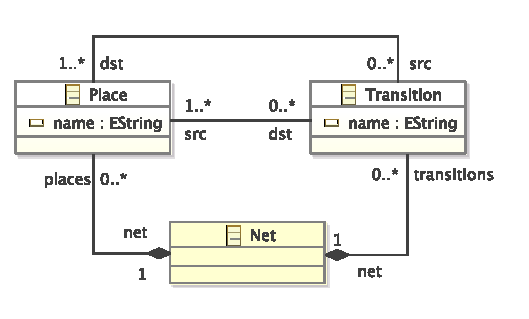
\includegraphics[scale=0.75]{petri_nets_step0.pdf}
  \caption{Original Petri nets metamodel.}
  \label{fig:original_mm}
\end{figure}

The evolved metamodel is shown in Figure~\ref{fig:evolved_mm}. \texttt{Place}s are connected to \texttt{Transition}s via instances of \texttt{PTArc}. Likewise, \texttt{Transition}s are connected to \texttt{Place}s via \texttt{TPArc}. Both \texttt{PTArc} and \texttt{TPArc} inherit from \texttt{Arc}, and therefore can be used to specify a \texttt{weight}.

\begin{figure}[htbp]
  \centering
  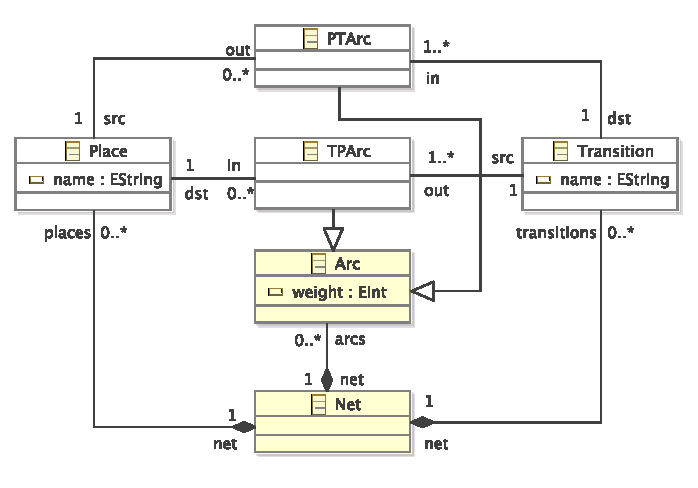
\includegraphics[scale=0.75]{petri_nets_step1.pdf}
  \caption{Evolved Petri nets metamodel.}
  \label{fig:evolved_mm}
\end{figure}

Models that were consistent with the original metamodel may not be consistent with the evolved metamodel. For example, \texttt{Transition} objects can no longer define values for \texttt{src} and \texttt{dst} features, and must define at least one value for the \texttt{in} and \texttt{out} features.

The migration strategy for this evolution varies when specified in ATL, Groovy-for-COPE and Flock, largely due to the differences in the way in which each approach initialises migrated models. When specified in ATL, migration must copy values from original to migrated model, as shown on lines 5-6, 12 and 20 of Listing~\ref{lst:quantitive_etl}. When using Groovy-for-COPE, values contained in slots that no longer correspond to features in the migrated metamodel must be unset, as shown on lines 2, 9 and 18-19 of Listing~\ref{lst:quantitive_cope}. Finally, Flock initialises the migrated model by copying values only for those features that remain unchanged in the migrated model. Consequently, no explicit copying or unsetting is required in Listing~\ref{lst:quantitive_flock}; the migration strategy manipulates only metafeatures that do not exist in the evolved metamodel (\texttt{Transition\#src} and \texttt{Transition\#dst}) and the new metaclasses, \texttt{TPArc} and \texttt{PTArc}.

\begin{lstlisting}[basicstyle=\ttfamily\footnotesize, flexiblecolumns=true, numbers=left, nolol=true, caption=Petri nets model migration in ATL, label=lst:quantitive_etl, language=ETL, tabsize=2]
rule Nets {
	from
		o : Before!Net
	to
	  m : After!Net ( places <- o.places, transitions <- o.transitions )
}

rule Places {
	from
		o : Before!Place
	to
		m : After!Place ( name <- o.name )
}

rule Transitions {
	from
		o : Before!Transition
	to
		m : After!Transition (
			name <- o.name,
			"in" <- o.src->collect(p | thisModule.PTArcs(p,o)),
			out  <- o.dst->collect(p | thisModule.TPArcs(o,p))
		)
}

lazy rule PTArcs {
	from
		place       : Before!Place,
		destination : Before!Transition
	to
		ptarcs : After!PTArc (
			src <- place,
			dst <- destination,
			net <- destination.net
		)
}

lazy rule TPArcs {
	from
		transition  : Before!Transition,
		destination : Before!Place
	to
		tparcs : After!TPArc (
			src <- transition,
			dst <- destination,
			net <- transition.net
		)
}
\end{lstlisting}


\begin{lstlisting}[basicstyle=\ttfamily\footnotesize, flexiblecolumns=true, numbers=left, nolol=true, caption=Petri nets model migration in COPE, label=lst:quantitive_cope, language=Java, tabsize=2]
for (transition in Transition.allInstances) {
  for (source in transition.unset('src')) {
    def arc = petrinets.PTArc.newInstance()
    arc.src = source
    arc.dst = transition
    arc.net = transition.net
  }

  for (destination in transition.unset('dst')) {
    def arc = petrinets.TPArc.newInstance() 
    arc.src = transition
    arc.dst = destination
    arc.net = transition.net
  }
}

for (place in Place.allInstances) {
  place.unset('src')
  place.unset('dst')
}
\end{lstlisting}


\begin{lstlisting}[basicstyle=\ttfamily\footnotesize, flexiblecolumns=true, numbers=left, nolol=true, caption=Petri nets model migration in Flock, label=lst:quantitive_flock, language=Flock, tabsize=2]
migrate Transition {
  for (source in original.src) {
    var arc := new Migrated!PTArc;
    arc.src := source.equivalent();
    arc.dst := migrated;
    arc.net := original.net.equivalent();
  }

  for (destination in original.dst) {
    var arc := new Migrated!TPArc;
    arc.src := migrated;
    arc.dst := destination.equivalent();
    arc.net := original.net.equivalent();
  }
}
\end{lstlisting}

With regard to the way in which they initialise the migrated model, COPE and ATL are opposites. The former initialises an exact copy of the original model, and so unset operations must be used when the value of a feature should not have been copied. By contrast, the latter initialises an empty model, and so explicit assignment operations must be used to copy values from original to migrated model for each feature that is not affected by the metamodel evolution.

This difference explains the results shown in Table~\ref{tab:model_operations_results}. Firstly, because Flock requires no unsetting of affected model elements nor explicit copying of unaffected model elements, less model operations are used when specifying a migration strategy with Flock than is used when specifying the same migration strategy with Groovy-for-COPE or with ATL. Secondly, there are more features unaffected by metamodel evolution than affected. Consequently, specifying model migration with ATL for the examples shown in Table~\ref{tab:model_operations_results} requires more model operations than in Groovy-for-COPE.


\paragrah{Side-Effects during Initialisation}
The measurements observed for one of the examples of co-evolution from Chapter~\ref{Analysis}, Change Reference to Containment, cannot be explained by the difference in copying strategy. Instead, the way in which models are initialised by the migration languages must be considered. When a reference feature is changed to a containment reference during metamodel evolution, constructing the migrated model by starting from the original model (as is the case with Groovy-for-COPE and, when the feature is not renamed, also Flock) can have side-effects which complicate migration.

In the Change Reference to Containment example, a \texttt{System} initially comprises \texttt{Port}s and \texttt{Signature}s (Figure~\ref{fig:ref2cont_original_mm}). A \texttt{Signature} references any number of \texttt{ports}. The metamodel is to be evolved so that \texttt{Port}s can no longer be shared between \texttt{Signature}s.

\begin{figure}[htbp]
  \centering
  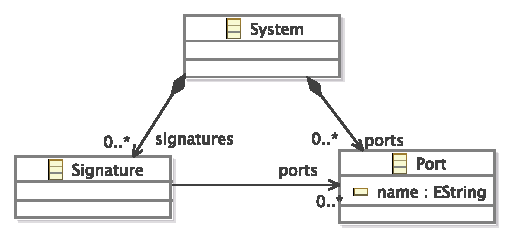
\includegraphics[scale=0.75]{change_ref_to_cont_before.pdf}
  \caption{Original metamodel.}
  \label{fig:ref2cont_original_mm}
\end{figure}

The evolved metamodel is shown in Figure~\ref{fig:ref2cont_evolved_mm}. \texttt{Signature}s now contain - rather than reference - \texttt{Port}s. Consequently, the \texttt{ports} feature of \texttt{System} is no longer required and is removed.

\begin{figure}[htbp]
  \centering
  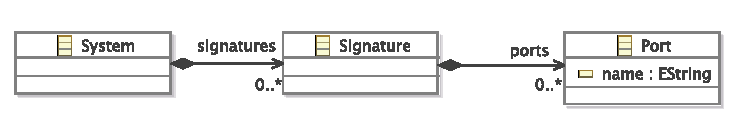
\includegraphics[scale=0.75]{change_ref_to_cont_after.pdf}
  \caption{Evolved metamodel.}
  \label{fig:ref2cont_evolved_mm}
\end{figure}

The migration strategy is straightforward in ATL: for each \texttt{Signature} in the original model, each member of the \texttt{ports} feature is cloned, using a lazy rule, and added to the \texttt{ports} feature of the equivalent \texttt{Signature}.

\begin{lstlisting}[basicstyle=\ttfamily\footnotesize, flexiblecolumns=true, numbers=left, nolol=true, caption=Change R to C model migration in ATL, label=lst:ref2cont_atl, language=ATL, tabsize=2]
rule Systems {
	from
		o : Before!System
	to
		m : After!System ( signatures <- o.signatures )
}

rule Signature {
	from
		o : Before!Signature
	to
		m : After!Signature (
			ports <- o.ports->collect(p | thisModule.Port(p))
		)
}

lazy rule Port {
	from
		o : Before!Port
	to
		m : After!Port ( name <- o.name )
\end{lstlisting}

In Flock and Groovy-for-COPE, migration is less straightforward because, during migration, the value of a containment reference (\texttt{Signature\#ports}) is set automatically by the migration strategy execution engine. When a containment reference is set, the contained objects are removed from their previous containment reference (i.e. setting a containment reference can have side-effects). Therefore, in a \texttt{System} where more than one \texttt{Signature} references the same \texttt{Port}, the migrated model cannot be formed by copying the contents of \texttt{Signature\#ports} from the original model. Attempting to do so causes each \texttt{Port} to be contained only in the last referencing \texttt{Signature} that was copied.

In Groovy-for-COPE, the containment nature of the reference is not enforced until after the migration strategy is executed. Hence, the migration strategy can be specified by unsetting the contents of the \texttt{ports} reference (line 4 of Listing~\ref{lst:ref2cont_cope}), and creating a copy of each referenced \texttt{Port} (lines 5-7 of Listing~\ref{lst:ref2cont_cope}). Unlike the ATL migration strategy, the ports in the Groovy-for-COPE migration strategy are cloned in the same model as the original port. Consequently, the Groovy-for-COPE migration strategy must either only clone ports that are referenced by more than one signature or clone every referenced port, but delete all of the original ports. The latter approach requires 2 more model operations (to populate and delete the original ports) than the former (shown in Listing~\ref{lst:ref2cont_cope}).

\begin{lstlisting}[basicstyle=\ttfamily\footnotesize, flexiblecolumns=true, numbers=left, nolol=true, caption=Change R to C model migration in COPE, label=lst:ref2cont_cope, language=COPE, tabsize=2]
def contained = []

for(signature in refactorings_changeRefToCont.Signature.allInstances) {
  for(port in signature.ports)) {
	  // when more than one Signature references this port
	  if (contained.contains(port)) {
      def clone = Port.newInstance()
      clone.name = port.name
      signature.ports.add(clone)
      signature.ports.remove(port)
		} else {
			contained.add(port)
		}
  }
}

for(port in refactorings_changeRefToCont.Port.allInstances) {
	if (not refactorings_changeRefToCont.Signature.allInstances.any { it.ports.contains(port) }) {
	  	port.delete()
	}
}
\end{lstlisting}

In Flock, the containment nature of the reference is enforced when the migrated model is initialised. Because changing the contents of a containment reference can have side-effects, a \texttt{Port} that appears in the \texttt{ports} reference of a \texttt{Signature} in the original model may not have been automatically copied to the \texttt{ports} reference of the equivalent \texttt{Signature} in the migrated model during initialisation. Consequently, the migration strategy must check the \texttt{ports} reference of each migrated \texttt{Signature}, cloning only those \texttt{Port}s that have not be automatically copied during initialisation (see line 3 of Listing~\ref{lst:ref2cont_flock}).

\begin{lstlisting}[basicstyle=\ttfamily\footnotesize, flexiblecolumns=true, numbers=left, nolol=true, caption=Change R to C model migration in Flock, label=lst:ref2cont_flock, language=Flock, tabsize=2]
migrate Signature {
	for (port in original.ports) {
		if (migrated.ports.excludes(port.equivalent())) {
			var clone := new Migrated!Port;
			clone.name := port.name;
			migrated.ports.add(clone);
		}
	}
}

delete Port when: not Original!Signature.all.exists(s|s.ports.includes(original))
\end{lstlisting}


The Groovy-for-COPE and Flock migration strategies must also remove any \texttt{Port}s which are not referenced by any \texttt{Signature} (lines 17-21 of Listing~\ref{lst:ref2cont_cope}, and line 11 of Listing~\ref{lst:ref2cont_flock} respectively), whereas the ATL migration strategy, which initialises any empty migrated model, does not copy unreferenced \texttt{Port}s.

When a non-containment reference is changed to a containment reference, a Flock migration strategy requires one more more model operation than the equivalent ATL migration strategy: to delete model elements that are not contained in any instance of the containment reference (line 11 of Listing~\ref{lst:ref2cont_flock}). A Groovy-for-COPE migration strategy requires three more model operations than the equivalent ATL migration strategy: one to delete model elements that are not contained in any instance of the containment reference (lines 17-21 of Listing~\ref{lst:ref2cont_cope}), one to dereference model elements that have already been cloned (line 10 of Listing~\ref{lst:ref2cont_cope}), and one to mark a model element as contained (line 12 of Listing~\ref{lst:ref2cont_cope}).  In the example considered here, the ATL migration strategy requires one more model operation than the Flock and Groovy-for-COPE migration strategies (to copy the contents of System\#signature features from original to migrated model), due to the difference in copying strategy. This leads to the result shown in Table~\ref{tab:model_operations_results}: the Flock and ATL migration strategies have an equal number of model operations, while the COPE migration strategy has two more.


\subsubsection{Summary}
This section has compared the model migration languages

- Make clear the contribution: no other research has attempted to compare model migration languages. It's not clear how it should be done. This is a start. 
- Not trying to argue that the figures are statistically significant. Just an approximation of what we're trying to measure.
- Extensions: measure cyclomatic complexity, etc




\section{Discussion}
% We will discuss the limitations of our work, using for context the feedback of users, reviews of publications and scenarios from the case study discussed in Section~\ref{subsubsec:case_study}

\subsection{Threats to validity}



\section{Dissemination / Reception / ??}

\subsection{Publications}
% Publication in academic journals, and at international conferences and workshops ensure that our work is reviewed by experts, and is well-established and communicated in our field of research. So far, I have been the primary author for publications at one international conference (\cite{rose08hutn}), one European conference (\cite{rose08egl}), and one workshop (\cite{rose09patterns}). The first was published at MoDELS/UML, the leading international conference on model-driven engineering, in a year when it had a record number of submissions (274, 20\% acceptance), and has been nominated by HISE for the annual departmental award for best paper by a research student.

% We will submit our work to software evolution conferences, as well as at model-driven engineering conferences. Doing so will allow us to assess the impact of our research for a broader audience.


\subsection{Delivery through Eclipse}
% The tools produced as part of our research have been and will continue to be released as part of the Epsilon project, a member of the research incubator for the Eclipse Modeling Project (EMP), arguably the most active MDE community at present. EMP's research incubator hosts a limited number of participants, selected through a rigorous process. Contributions made to the incubator undergo regular technical review.

% Contributing to Epsilon allows us to deliver our research to the growing community \cite{kolovos08thesis} of Epsilon users.
